\begin{exercises} 
\item This problem concerns a function about which the following information is known:
\begin{itemize}
	\item $f$ is a differentiable function defined at every real number $x$
	\item $f(0) = -1/2$
	\item $y = f'(x)$ has its graph given at center in Figure~\ref{F:3.1.Ez1}
\end{itemize}
\begin{figure}[h]
\begin{center}
\scalebox{0.9}{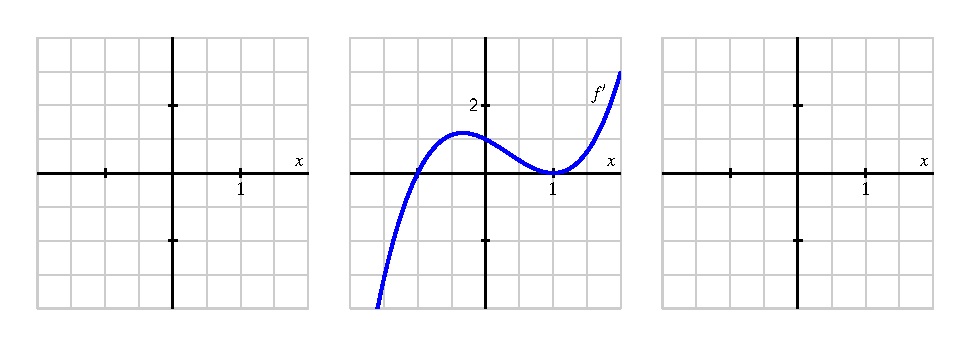
\includegraphics{figures/3_1_Ez1.eps}}
\end{center}
\caption{At center, a graph of $y = f'(x)$; at left, axes for plotting $y = f(x)$; at right, axes for plotting $y = f''(x)$.} \label{F:3.1.Ez1}
\end{figure}
\ba
	\item Construct a first derivative sign chart for $f$.  Clearly identify all critical numbers of $f$, where $f$ is increasing and decreasing, and where $f$ has local extrema.
	\item On the right-hand axes, sketch an approximate graph of $y = f''(x)$.
	\item Construct a second derivative sign chart for $f$.  Clearly identify where $f$ is concave up and concave down, as well as all inflection points.
	\item On the left-hand axes, sketch a possible graph of $y = f(x)$.
\ea

\item Suppose that $g$ is a differentiable function and $g'(2) = 0$.  In addition, suppose that on $1 < x< 2$ and $2 < x < 3$ it is known that $g'(x)$ is positive.
\ba
	\item Does $g$ have a local maximum, local minimum, or neither at $x = 2$?  Why?
	\item Suppose that $g''(x)$ exists for every $x$ such that $1 < x < 3$.  Reasoning graphically, describe the behavior of $g''(x)$ for $x$-values near $2$.
	\item Besides being a critical number of $g$, what is special about the value $x = 2$ in terms of the behavior of the graph of $g$?
\ea

\item Suppose that $h$ is a differentiable function whose first derivative is given by the graph in Figure~\ref{F:3.1.Ez3}.
\begin{figure}[h]
\begin{center}
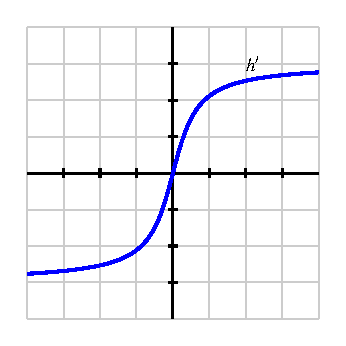
\includegraphics{figures/3_1_Ez3.eps}
\end{center}
\caption{The graph of $y = h'(x)$.} \label{F:3.1.Ez3}
\end{figure}
\ba
	\item How many real number solutions can the equation $h(x) = 0$ have?  Why?
	\item If $h(x) = 0$ has two distinct real solutions, what can you say about the signs of the two solutions?  Why?
	\item Assume that $\lim_{x \to \infty} h'(x) = 3$, as appears to be indicated in Figure~\ref{F:3.1.Ez3}.  How will the graph of $y = h(x)$ appear as $x \to \infty$?  Why?
	\item Describe the concavity of $y = h(x)$ as fully as you can from the provided information.
\ea

\item Let $p$ be a function whose second derivative is $p''(x) = (x+1)(x-2)e^{-x}$.
	\ba
		\item Construct a second derivative sign chart for $p$ and determine all inflection points of $p$.
		\item Suppose you also know that $x = \frac{\sqrt{5}-1}{2}$ is a critical number of $p$.  Does $p$ have a local minimum, local maximum, or neither at $x = \frac{\sqrt{5}-1}{2}$?  Why?
		\item If the point $(2, \frac{12}{e^2})$ lies on the graph of $y = p(x)$ and $p'(2) = -\frac{5}{e^2}$, find the equation of the tangent line to $y = p(x)$ at the point where $x = 2$.  Does the tangent line lie above the curve, below the curve, or neither at this value?  Why?
	\ea
\end{exercises}
\afterexercises